\begin{figure}[t]
  \centering
  \begin{subfigure}[b]{0.266\textwidth}
    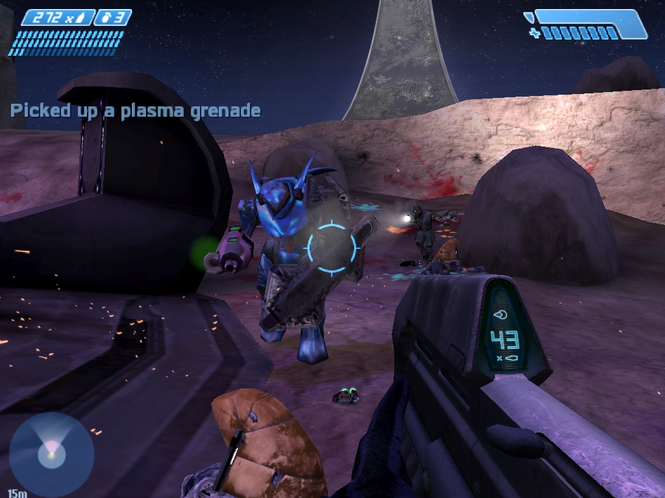
\includegraphics[width=\textwidth]{./img/raw/intro-halo/halo_1.png}
    \caption{Halo 1: 2001.}
    \label{fig:intro-halo:1}
  \end{subfigure} \quad
  \begin{subfigure}[b]{0.25\textwidth}
    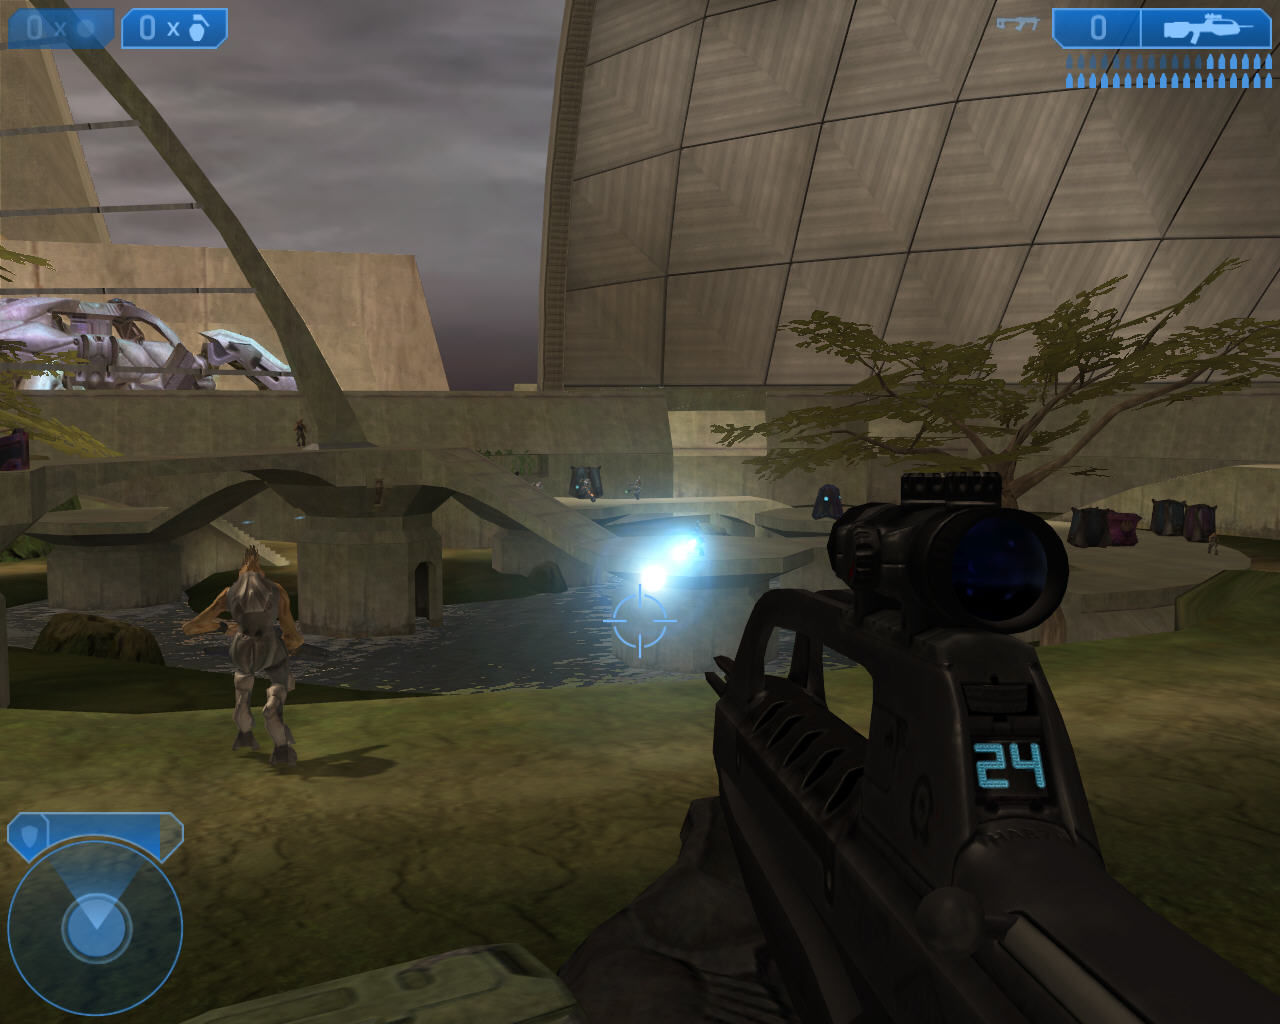
\includegraphics[width=\textwidth]{./img/raw/intro-halo/halo_2.png}
    \caption{Halo 2: 2004.}
    \label{fig:intro-halo:2}
  \end{subfigure} \quad
  \begin{subfigure}[b]{0.356\textwidth}
    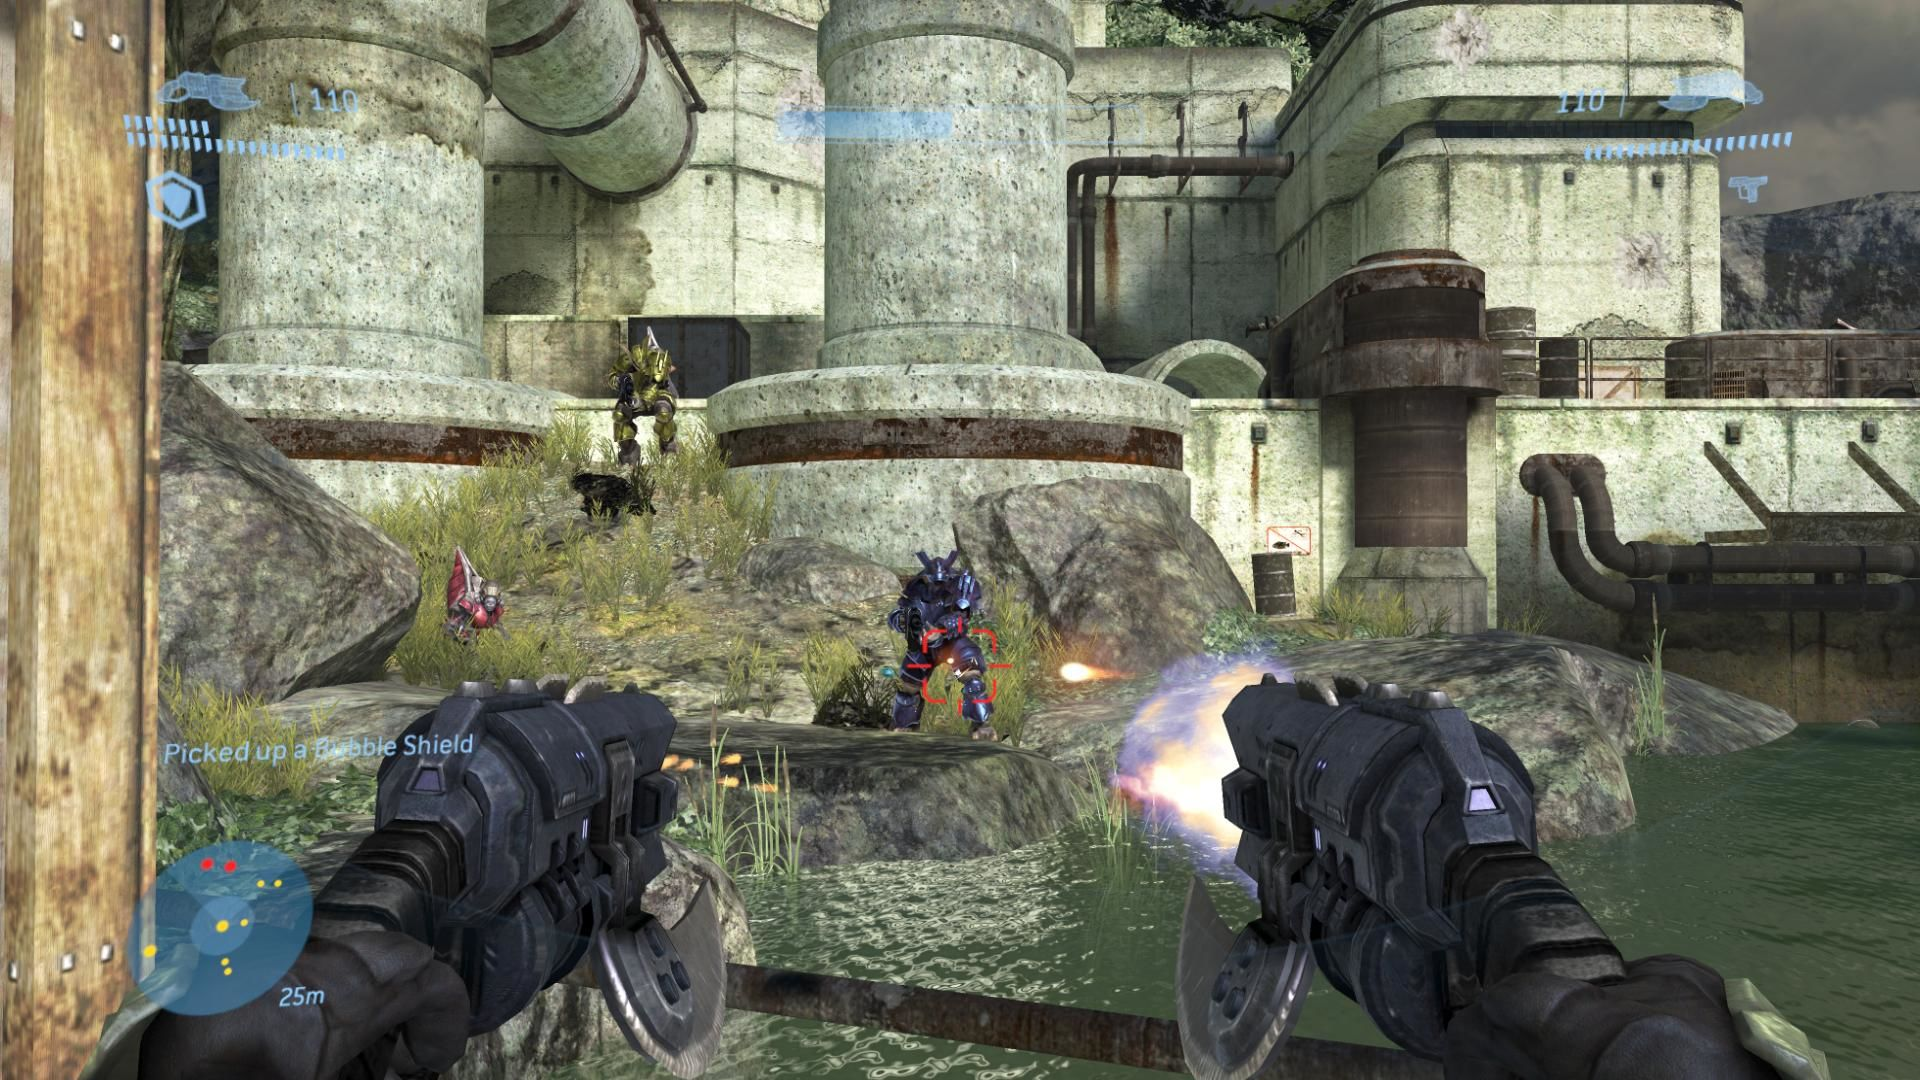
\includegraphics[width=\textwidth]{./img/raw/intro-halo/halo_3.png}
    \caption{Halo 3: 2007.}
    \label{fig:intro-halo:3}
  \end{subfigure}\\
  \begin{subfigure}[b]{0.45\textwidth}
    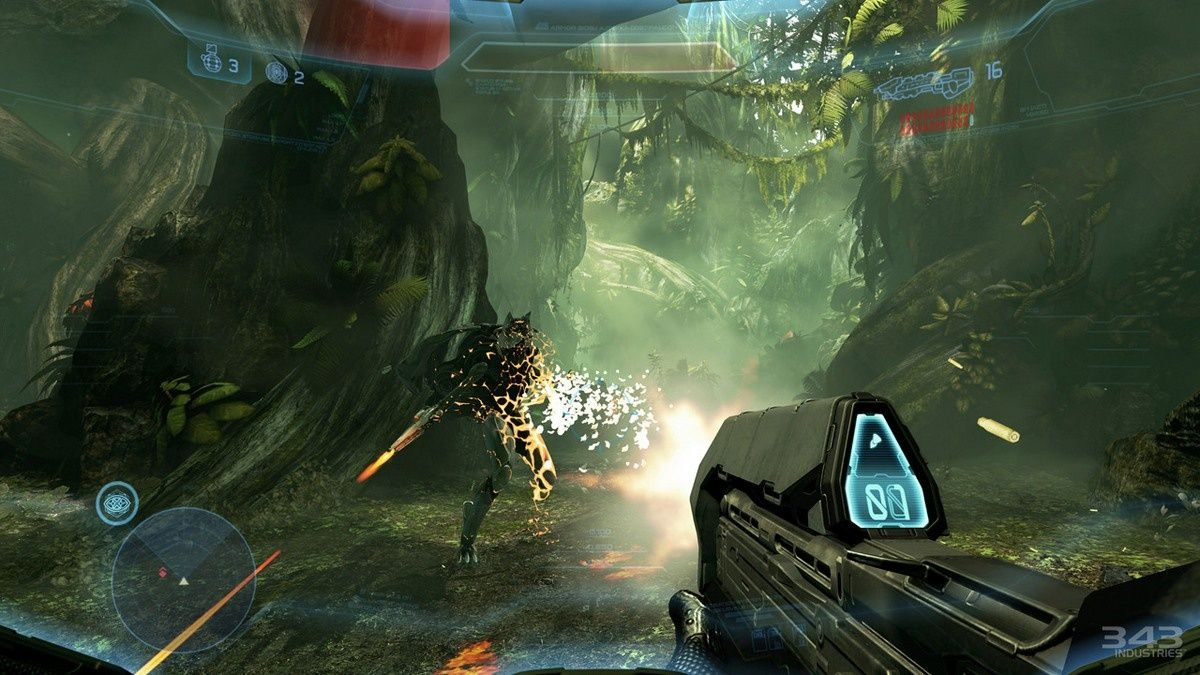
\includegraphics[width=\textwidth]{./img/raw/intro-halo/halo_4.jpg}
    \caption{Halo 4: 2012.}
    \label{fig:intro-halo:4}
  \end{subfigure} \quad
  \begin{subfigure}[b]{0.45\textwidth}
    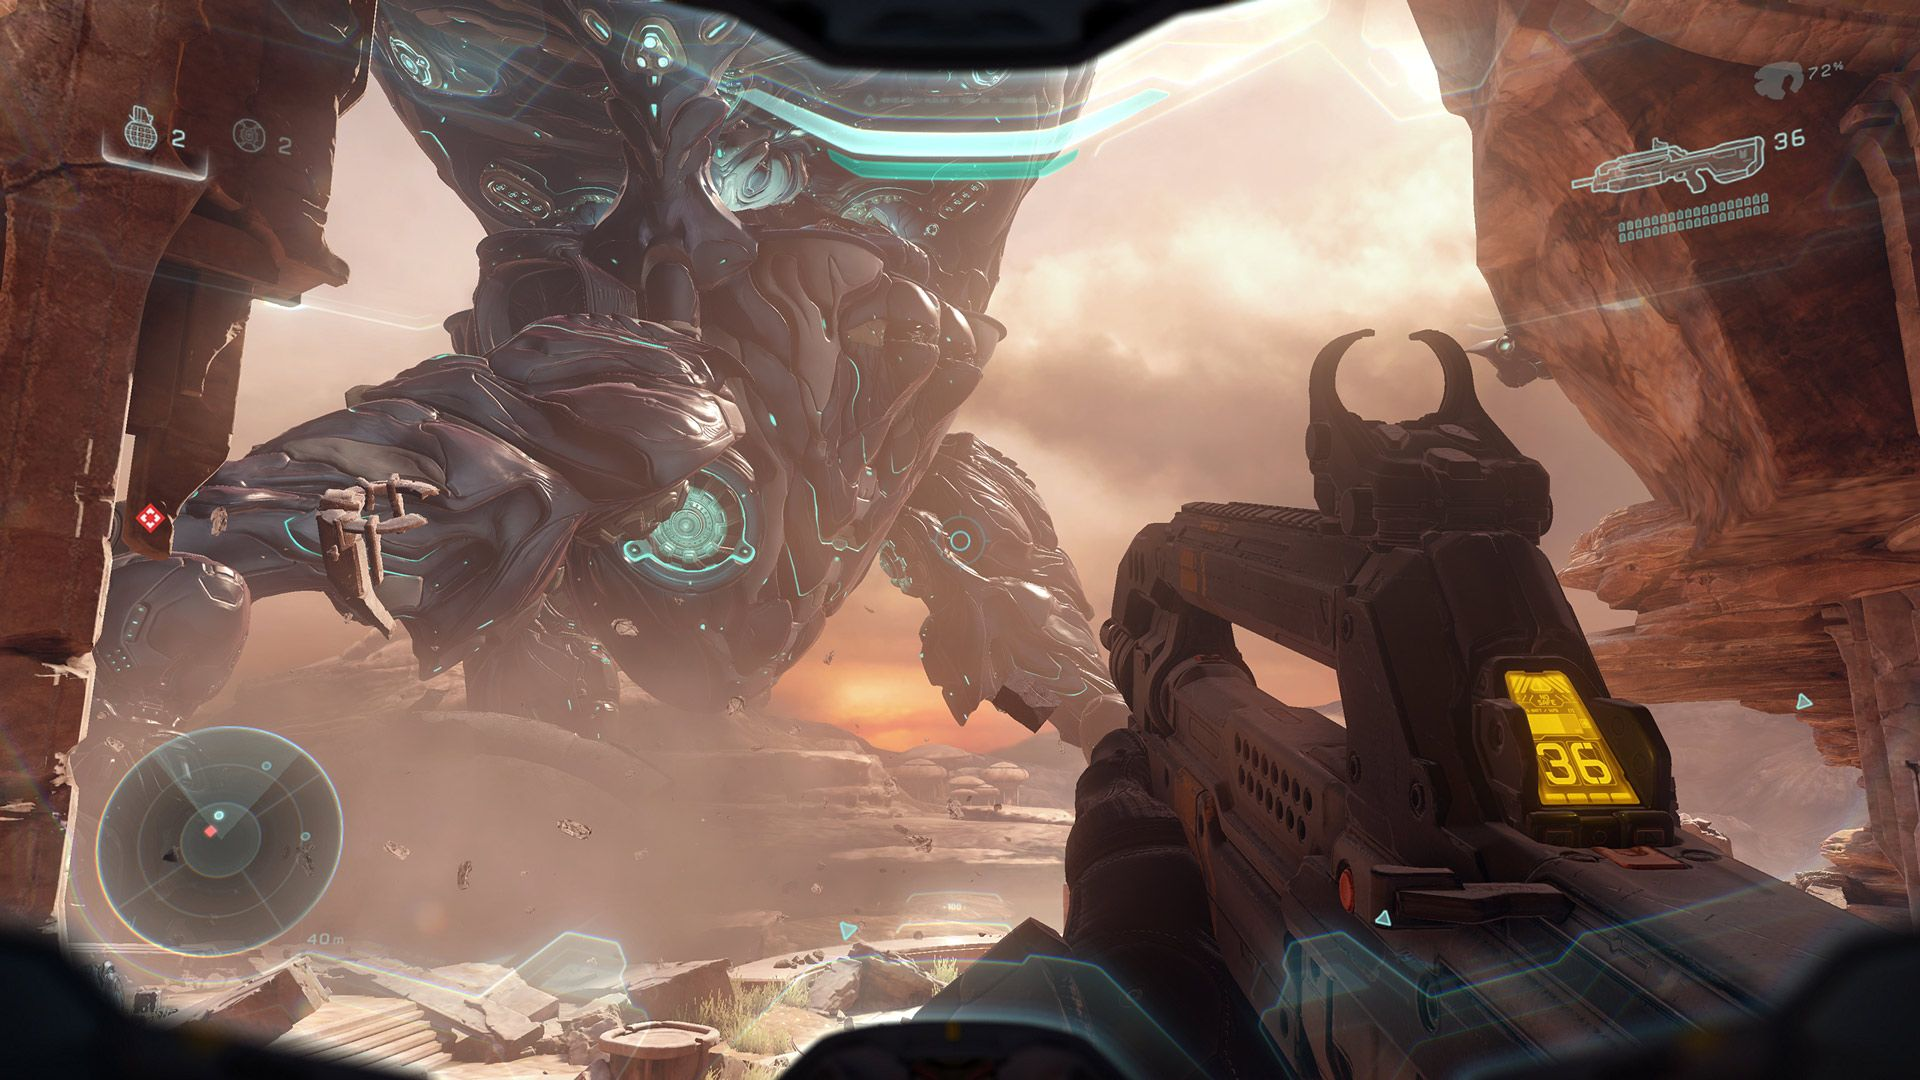
\includegraphics[width=\textwidth]{./img/raw/intro-halo/halo_5.jpg}
    \caption{Halo 5: 2015.}
    \label{fig:intro-halo:5}
  \end{subfigure}
  \caption{Progressie van grafische kwaliteit in de Halo series.}
  \label{fig:intro-halo}
\end{figure}
